
\newcolumntype{a}{>{\columncolor{RoyalBlue!50}}l}
\newcolumntype{b}{>{\columncolor{RoyalBlue!50}}p{1.2cm}}
\newcolumntype{d}{>{\columncolor{RoyalBlue!50}}p{.6cm}}
\newcolumntype{R}[1]{%
    >{\columncolor{RoyalBlue!50}\adjustbox{angle=#1}\bgroup}%
    l<{\egroup}|%
}
\newcommand*\rotCol{\multicolumn{1}{R{90}}}

\lstset{style=sql, basicstyle=\ttfamily\scriptsize}

\lstset{style=sql, basicstyle=\ttfamily\scriptsize}

\title[Datenbanken] {Datenbanken}

\subtitle{\emoji{floppy-disk} \textbf{\gls{SQL}: mehrere Tabellen}}

\author[Blum, Cyril] % (optional)
{Naoki Peter\inst{1} \and Cyril Blum \inst{2}}

\institute[KZN] % (optional)
{
  \inst{1}%
  Fachschaft Informatik\\
  Kantonsschule Zürich-Nord
  \and
  \inst{2}%
  Fachschaft Informatik\\
  Kantonsschule im Lee
}

\date[\today] % (optional)

\logo{
\includegraphics[width=.8cm]{Logos/LeeLogo}}

\titlegraphic{\includegraphics[width=\textwidth]{"Grundlagen_Info/06_Datenbanken/Figures/title-emojis"}}

\frame{\titlepage}


\begin{frame}[fragile]{Weshalb braucht es mehrere Tabellen?}{Analogie: Wörterbuch}
Angenommen, Sie lesen einen Text in deutscher Sprache. Wäre es praktisch, wenn jedes Wort in einer Klammer erklärt wäre?\\[.5cm]


\begin{tcolorboxTemplate}[title=Beispiel]
\tiny\textbf{Ich} (\enquote{das Selbst, dessen man sich bewusst ist und mit dem man sich von der Umwelt unterscheidet}) \textbf{ging} (gehen, \enquote{schrittweises Sichfortbewegen auf den Füssen in aufrechter Haltung}) \textbf{nach} (\enquote{drückt aus, dass jemand jemandem, einer Sache folgt, nachgeht}) \textbf{draussen} (\enquote{ausserhalb eines Raumes, Gebäudes})...
\end{tcolorboxTemplate}


\normalsize
Alternative: Nachschlagewerk / Wörterbuch!

\end{frame}

\begin{frame}[fragile]{Weshalb braucht es mehrere Tabellen?}{Analogie: Soziale Medien}
\begin{center}
Wäre es praktisch, wenn Sie bei Ihrer Tiktok-Freundesliste immer auch gleich all deren Posts, Kommentare und alles Weitere sehen könnten?
\end{center}
\end{frame}

\begin{frame}{Tabellen-Organisation}
\Wider{\begin{figure}[H]
\centering
\includegraphics[width=\linewidth]{"Grundlagen_Info/06_Datenbanken/Figures/schema MM"}
\end{figure}}
\begin{itemize}
\item Was bedeuten die blauen Pfeile und die Schlüssel?
\end{itemize}
\end{frame}


\begin{frame}[fragile]{Primärschlüssel einer Tabelle}

\begin{table}
\centering
\begin{tabular}{a|l|l}
\emoji{key} \underline{mID} & Name   & ... \\\midrule
1  & Müller  & ...  \\
2  & Schmidt & ...  \\
3  & Kaufmann  & ...\\
... & ... & ... 
\end{tabular}
\caption*{Tabelle \enquote{\textbf{Angestellte}}}
\end{table}
\begin{center}
\textbf{Frage}: Weshalb hat (fast) jede Tabelle einen Primärschlüssel \emoji{key}?
\end{center}
\end{frame}

\begin{frame}[fragile]{Fremdschlüssel einer Tabelle}

\begin{columns}
\begin{column}{.5\textwidth}
\begin{table}[H]
\begin{tabular}{l|l|a}
\emoji{key} \underline{mID} & Name   & \tikzmarknode{fkey}{\underline{aID} \emoji{up-right-arrow}} \\\midrule
1  & Müller  & \tikzmarknode{31o}{31}  \\
2  & Schmidt & \tikzmarknode{32o1}{32}  \\
3  & Kaufmann  & \tikzmarknode{32o2}{32}\\
... & ... & ... 
\end{tabular}
\caption*{Tabelle \enquote{\textbf{Angestellte}}}
\end{table}
\end{column}
\begin{column}{.5\textwidth}
\begin{table}[H]
\begin{tabular}{a|l}
\tikzmarknode{pkey}{\emoji{key} \underline{aID}} & Abteilungs \\\midrule
\tikzmarknode{31t}{31}    & Verkauf   \\
\tikzmarknode{32t}{32}    & Technik   \\
\tikzmarknode{33t}{33}    & Marketing \\
... & ... 
\end{tabular}
\caption*{Tabelle \enquote{\textbf{Abteilungen}}}
\end{table}
\end{column}
\end{columns}


\only<2->{
\begin{tikzpicture}[overlay,remember picture]
% title
 \draw[red,-stealth] (fkey) to[bend left] (pkey);
% values
  \draw[red,-stealth] (31o) -- (31t);
  \draw[red,-stealth] (32o1) -- (32t);
  \draw[red,-stealth] (32o2) -- (32t);
\end{tikzpicture}}

\begin{center}
\only<1>{
\textbf{Frage}: Was könnte ein Fremdschlüssel \emoji{up-right-arrow} sein? \\

Weshalb könnten Fremdschlüssel benötigt werden?
}
\only<2>{
\textbf{Frage}: Was ist die Abteilung von Frau Kaufmann?
}
\end{center}

\end{frame}

\begin{frame}[fragile]{Mehrere Tabellen miteinander verbinden}{Möglichkeit 2b: Verwendung von \lstinline[style=sql]|JOIN| (mit \lstinline[style=sql]|ON|, falls Kolonnennamen ungleich)}
	\begin{lstlisting}
		SELECT *
		FROM Angestellte JOIN Abteilung
		ON Angestellte.aID = Abteilung.ID
	\end{lstlisting}
	\vspace{-.3cm}
	\footnotesize
	\begin{columns}
		\begin{column}{.35\textwidth}
			\begin{table}[H]
				\begin{tabular}{l|l|a}
					\emoji{key} \underline{mID} & Name   & \underline{aID} \emoji{up-right-arrow} \\\midrule
					1  & Müller  & 31  \\
					2  & Schmidt & 32  \\
					3  & Kaufmann  & 32\\
					... & ... & ... 
				\end{tabular}
				\caption*{Tabelle \enquote{\textbf{Angestellte}}}
			\end{table}
			\vspace{-.5cm}\begin{table}[H]
				\begin{tabular}{a|l}
					\emoji{key} \underline{ID} & Abteilungs \\\midrule
					31    & Verkauf   \\
					32    & Technik   \\
					33    & Marketing \\
					... & ... 
				\end{tabular}
				\caption*{Tabelle \enquote{\textbf{Abteilungen}}}
			\end{table}
			
		\end{column}
		\begin{column}{.1\textwidth}
			\faArrowRight
		\end{column}
		\begin{column}{.55\textwidth}
			\begin{table}[H]
				\begin{tabular}{l|l|a|a|l}
					mID & Name   & \rotCol{Angestellte.aID} & \rotCol{Abteilung.ID} & Abteilung \\\midrule
					1  & Müller  & 31  &31  & Verkauf\\
					2  & Schmidt & 32 &32 & Technik\\
					3  & Kaufmann  & 32 &32 & Technik \\
					... & ... & ... & ... 
				\end{tabular}
			\end{table}
		\end{column}
	\end{columns}
\end{frame}

\begin{frame}[fragile]{Verteilte Tabellen}


\begin{table}[H]
\centering
\tiny
\resizebox{\textwidth}{!}{
\begin{tabular}{l|p{7cm}}
\textbf{Tabelle} & \textbf{Spalten} \\\midrule\midrule
Lieferant&	\emoji{key} LieferantenNr, Firma, Kontaktperson, Position, Strasse, Ort, Region, PLZ, Land, Telefon, Telefax, Homepage\\\midrule
Kunde &	\emoji{key} KundenCode, Firma, Kontaktperson, Position, Strasse, Ort, Region, PLZ, Land, Telefon, Telefax\\\midrule
Versandfirma &	\emoji{key} FirmenNr, Firma, Telefon\\\midrule
Personal &	\emoji{key} PersonalNr, Nachname, Vorname, Position, Anrede, Geburtsdatum, Einstellung, Strasse, Ort, Region, PLZ, Land, TelefonPrivat, DurchwahlBüro, Bemerkungen, Vorgesetzter\\\midrule
Kategorie 	&\emoji{key} KategorieNr, Kategoriename, Beschreibung\\\midrule
Artikel 	&\emoji{key} ArtikelNr, Artikelname, LieferantenNr \emoji{up-right-arrow}, KategorieNr \emoji{up-right-arrow}, Liefereinheit, Einzelpreis, Lagerbestand, BestellteEinheiten, Mindestbestand, Auslaufartikel\\\midrule
Bestellung 	& \emoji{key} BestellNr, KundenCode \emoji{up-right-arrow}, PersonalNr \emoji{up-right-arrow}, Bestelldatum, Lieferdatum, Versanddatum, FirmenNr \emoji{up-right-arrow}, Frachtkosten, Empfänger, Strasse, Ort, Region, PLZ Bestimmungsland\\\midrule
Bestelldetails &	BestellNr \emoji{up-right-arrow}, ArtikelNr \emoji{up-right-arrow}, Einzelpreis, Anzahl, Rabatt
\end{tabular}}
\end{table}
\vspace{-.3cm}
\begin{figure}[H]
\centering

\includegraphics[width=0.3\linewidth]{Grundlagen_Info/06_Datenbanken/Figures/Migros}

\includegraphics[width=0.22\linewidth]{Grundlagen_Info/06_Datenbanken/Figures/Coop}
\end{figure}

\end{frame}


\begin{frame}{Auftrag: Moodle}
Verbinden von Tabellen aus der Nordwind-Datenbank
\end{frame}

\begin{frame}{Appendix}
\end{frame}
%
%\begin{frame}[fragile]
%  \begin{center}
%    Demo: InstaHub
%  \end{center}
%\end{frame}
%
%\begin{frame}[fragile]{Auftrag}
%  Skript (Moodle)
%  \begin{itemize}
%    \item \aufgabebox{Aufgabe(n) 1.38 (externer Link)}
%    \item \challengebox{Aufgaben im Skript, Kapitel 1.5}
%    \item \challengebox{Abgabe auf Moodle (InstaHub, \enquote{\lstinline[style=sql]|JOIN|})}
%  \end{itemize}
%\end{frame}
%
%
%\begin{frame}[fragile]{\lstinline[style=sql]|JOIN|-Typen}
%  \begin{figure}[htbp]
%    \centering
%
%    % INNER JOIN
%    \begin{subfigure}[b]{0.45\textwidth}
%      \centering
%      \begin{tikzpicture}
%        \tikzset{circle node/.style={circle,draw=black, fill=none, minimum size=25mm, inner sep=0pt}}
%        \node[circle node] (left) at (0,0) {};
%        \node[circle node] (right) at (1.5,0) {};
%        \begin{scope}
%          \clip (0,0) circle (1.25cm);
%          \fill[gray] (1.5,0) circle (1.25cm);
%        \end{scope}
%      \end{tikzpicture}
%      \caption{\lstinline[style=sql]|INNER JOIN|}
%    \end{subfigure}
%    \hfill
%    % LEFT OUTER JOIN
%    \begin{subfigure}[b]{0.45\textwidth}
%      \centering
%      \begin{tikzpicture}
%        \tikzset{circle node/.style={circle,draw=black, fill=none, minimum size=25mm, inner sep=0pt}}
%        \node[circle node] (left) at (0,0) {};
%        \node[circle node] (right) at (1.5,0) {};
%        \begin{scope}
%          \clip (-1.5,-1.25) rectangle (1.25,1.25);
%          \fill[gray] (0,0) circle (1.25cm);
%        \end{scope}
%        \begin{scope}
%          \clip (0,0) circle (1.25cm);
%          \fill[gray] (1.5,0) circle (1.25cm);
%        \end{scope}
%      \end{tikzpicture}
%      \caption{\lstinline[style=sql]|LEFT OUTER JOIN|}
%    \end{subfigure}
%
%    \bigskip
%
%    % RIGHT OUTER JOIN
%    \begin{subfigure}[b]{0.45\textwidth}
%      \centering
%      \begin{tikzpicture}
%        \tikzset{circle node/.style={circle,draw=black, fill=none, minimum size=25mm, inner sep=0pt}}
%        \node[circle node] (left) at (0,0) {};
%        \node[circle node] (right) at (1.5,0) {};
%        \begin{scope}
%          \clip (0,-1.25) rectangle (4,1.25);
%          \fill[gray] (1.5,0) circle (1.25cm);
%        \end{scope}
%        \begin{scope}
%          \clip (1.5,0) circle (1.25cm);
%          \fill[gray] (0,0) circle (1.25cm);
%        \end{scope}
%      \end{tikzpicture}
%      \caption{\lstinline[style=sql]|RIGHT OUTER JOIN|}
%    \end{subfigure}
%    \hfill
%    % FULL OUTER JOIN
%    \begin{subfigure}[b]{0.45\textwidth}
%      \centering
%      \begin{tikzpicture}
%        \tikzset{circle node/.style={circle,draw=black, fill=none, minimum size=25mm, inner sep=0pt}}
%        \node[circle node] (left) at (0,0) {};
%        \node[circle node] (right) at (1.5,0) {};
%        \fill[gray] (0,0) circle (1.25cm);
%        \fill[gray] (1.5,0) circle (1.25cm);
%      \end{tikzpicture}
%      \caption{\lstinline[style=sql]|FULL OUTER JOIN|}
%    \end{subfigure}
%    \caption{Venn-Diagramme unterschiedlicher SQL-Joins}
%    \label{fig:venn-joins}
%  \end{figure}
%\end{frame}
%
%\begin{frame}{Weitere Beispiele}{Supermarkt}
%	\begin{center}
%		Was bevorzugen Sie?
%	\end{center}
%	\begin{table}[H]
%		\centering
%		\tiny
%		\begin{tabular}{l|p{1.2cm}|l|l|a|a|b}
%			\textbf{ArtikelNr} & \textbf{Artikelname}                     & \textbf{Einzelpreis} & \textbf{Lagerbestand} & \textbf{KategorieNr} & \textbf{Kategoriename} & \textbf{Beschreibung}                             \\\midrule
%			1         & Chai                            & 18.00       & 39           & 1           & Getränke      & Alkoholfreie Getränke, Kaffee, Tee, Bier \\\hline
%			2         & Chang                           & 19.00       & 17           & 1           & Getränke      & Alkoholfreie Getränke, Kaffee, Tee, Bier \\\hline
%			3         & Aniseed Syrup                   & 10.00       & 13           & 2           & Gewürze       & Süsse und saure Sossen, Gewürze            \\\hline
%			4         & Chef Anton's Cajun Seasoning    & 22.00       & 53           & 2           & Gewürze       & Süsse und saure Sossen, Gewürze            \\\hline
%			5         & Chef Anton's Gumbo Mix          & 21.35       & 0            & 2           & Gewürze       & Süsse und saure Sossen, Gewürze            \\\hline
%			6         & Grandma's Boysenberry Spread    & 25.00       & 120          & 2           & Gewürze       & Süsse und saure Sossen, Gewürze            \\\hline
%			…         & …                               & …           & …            & …           & …             & …                                       
%		\end{tabular}
%	\end{table}
%\end{frame}
%
%\begin{frame}{Weitere Beispiele}{Supermarkt}
%	\begin{center}
%		Was bevorzugen Sie?
%	\end{center}
%	
%	\begin{columns}
%		\begin{column}{.6\textwidth}
%			\begin{table}[H]
%				\tiny\centering
%				\begin{tabular}{@{}p{.6cm}|p{1.2cm}|p{.6cm}|p{.6cm}|b@{}}
%					\toprule
%					\textbf{ArtikelNr} & \textbf{Artikelname}         & \textbf{Einzelpreis} & \textbf{Lagerbestand} & \textbf{KategorieNr} \\ \midrule
%					1                  & Chai                         & 18.00                & 39                    & 1                    \\\hline
%					2                  & Chang                        & 19.00                & 17                    & 1                    \\\hline
%					3                  & Aniseed Syrup                & 10.00                & 13                    & 2                    \\\hline
%					4                  & Chef Anton's Cajun Seasoning & 22.00                & 53                    & 2                    \\\hline
%					5                  & Chef Anton's Gumbo Mix       & 21.35                & 0                     & 2                    \\\hline
%					6                  & Grandma's Boysenberry Spread & 25.00                & 120                   & 2                    \\\hline
%					…                  & …                            & …                    & …                     & …                    \\
%					\bottomrule
%				\end{tabular}
%			\end{table}
%		\end{column}
%		\begin{column}{.4\textwidth}
%			\begin{table}[H]
%				\tiny\centering
%				\begin{tabular}{@{}b|p{1.2cm}|p{1.2cm}@{}}
%					\toprule
%					\textbf{KategorieNr} & \textbf{Kategoriename}    & \textbf{Beschreibung}                             \\\midrule
%					1           & Getränke         & Alkoholfreie Getränke, Kaffee, Tee, Bier \\\hline
%					2           & Gewürze          & Süsse und saure Sossen, Gewürze            \\\hline
%					3           & Süsswaren         & Desserts und Süssigkeiten                 \\\hline
%					4           & Milchprodukte    & Käsesorten                               \\\hline
%					5           & Getreideprodukte & Brot, Kräcker, Nudeln, Müsli             \\\hline
%					6           & Fleischprodukte  & Fleisch-Fertiggerichte                   \\\hline
%					7           & Naturprodukte    & Getrocknete Früchte, Tofu usw.           \\\hline
%					8           & Meeresfrüchte    & Meerespflanzen und -früchte, Fisch      \\\bottomrule
%				\end{tabular}
%			\end{table}
%		\end{column}
%	\end{columns}
%\end{frame}
%
%\begin{frame}[fragile]{Eine Schul-Datenbank}
%  Eine Schule möchte eine Datenbank entwerfen. Sie will folgende Informationen speichern:
%  \begin{itemize}
%    \item SchülerInnen: Namen, Geschlecht, Geburtsdatum, Wohnort
%    \item LehrerInnen: Namen, Geschlecht, Geburtsdatum, Wohnort, Gehalt, Fach (oder Fächer), Klasse (oder Klassen)
%    \item Klassen: SchülerInnen, Klassenname, Klassenlehrperson
%  \end{itemize}
% Wäre es praktisch, wenn wir all diese Informationen in einer Tabelle hätten?
% \only<2>{
%\begin{itemize}
%	\item Unübersichtlich
%	\item Redundant (viele doppelte Werte)
%\end{itemize}}
%  \only<3->{
%    \begin{figure}[H]
%      \centering
%      \resizebox{\textwidth}{!}{%
%        \begin{tikzpicture}
%          % Entitäten
%          \node[entity] (lehrer) at (0,0) {Lehrer};
%          \node[entity] (schueler) at (14,0) {Schüler};
%          \node[entity] (klasse) at (7,0) {Klasse};
%
%          % Beziehungen
%          \node[relationship] (unterrichtet) at (3.5,0) {unterrichtet};
%          \node[relationship] (gehoert_zu) at (10.5,0) {gehört zu};
%
%          % Kanten
%          \draw (lehrer) -- (unterrichtet) node[midway,above]{n};
%          \draw (unterrichtet) -- (klasse) node[midway,above]{0:1};
%          \draw (schueler) -- (gehoert_zu) node[midway,above]{1};
%          \draw (gehoert_zu) -- (klasse) node[midway,above]{m};
%        \end{tikzpicture}
%      }
%    \end{figure}
%    \begin{mycaution}
%      Was bedeuten die Zahlen in der Zeichnung? Stimmen sie?
%    \end{mycaution}
%  }
%\end{frame}
%
%\begin{frame}{Weitere Beispiele}{Supermarkt}
%  \begin{figure}[H]
%    \centering
%    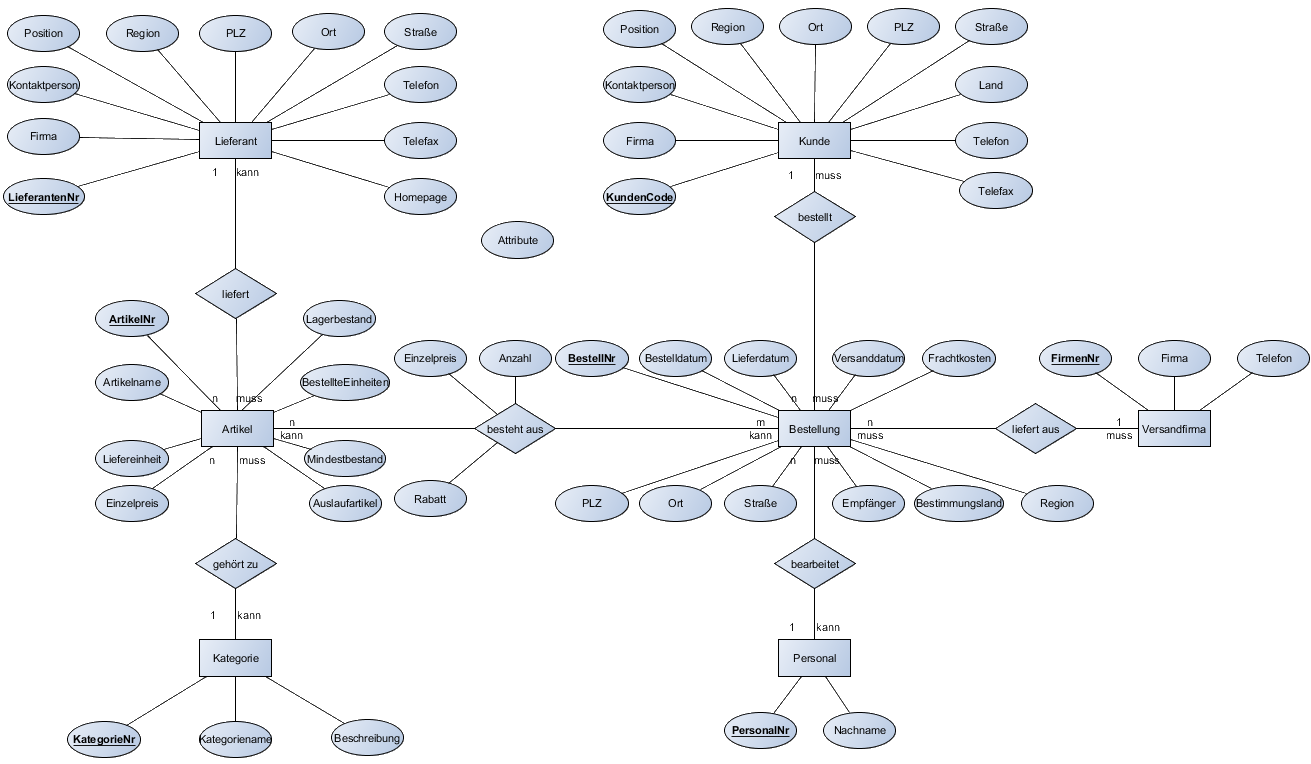
\includegraphics[width=\linewidth]{Grundlagen_Info/06_Datenbanken/Figures/er_nordwind_komplett}
%    \caption{Datenbank einer Firma, die Produkte verkauft (z.B. Supermarkt)}
%  \end{figure}
%
%\end{frame}
%
%
%\begin{frame}[fragile]{Was ist ein \gls{ERM}?}
%  \begin{figure}[H]
%    \centering
%    \resizebox{\textwidth}{!}{%
%      \begin{tikzpicture}[node distance=1cm]
%
%        % Entity
%        \node[entity] (entity1) {Entity};
%        \node[attribute] (attr1) [above left=of entity1] {Attribute} edge (entity1);
%        \node[attribute] (attr2) [below left=of entity1] {Attribute} edge (entity1);
%
%        % Relationship
%        \node[relationship] (rel1) [right=3cm of entity1] {Relationship} edge node[auto,swap] {n} (entity1);
%        \node[entity] (entity2) [right=3cm of rel1] {Entity} edge node[auto,swap] {m} (rel1);
%        \node[attribute] (attr3) [above=of rel1] {Attribute} edge (rel1);
%
%        % Legend
%        \node[draw,thick,fit=(entity1) (attr1) (attr2),inner sep=0.5cm, rounded corners, dotted, red] (box1) {};
%        \node[anchor=south, red] at (box1.north) {Einheiten (\textit{Entities}) und Attribute};
%
%        \node[draw,thick,fit=(rel1) (entity2) (attr3),inner sep=0.5cm, rounded corners, dotted, blue] (box2) {};
%        \node[anchor=south, blue] at (box2.north) {Beziehungen (\textit{Relationships})};
%
%      \end{tikzpicture}}
%    \caption{\gls{ERM}-Komponenten in der sogenannten Chen-Notation}
%    \label{fig:erm-components}
%  \end{figure}
%\end{frame}
%
%\begin{frame}[fragile]{\gls{ERM} von InstaHub}
%  \begin{figure}[H]
%    \centering
%    \resizebox{\textwidth}{!}{%
%      \begin{tikzpicture}[auto]
%        % Nodes
%        \node[entity] (user) at (0,0) {users};
%        \node[relationship] (follows) at (-4,0) {follows};
%        \node[relationship] (owns) at (2.5,2.5) {owns};
%        \node[entity] (photo) at (5,0) {photos};
%        \node[relationship] (has) at (7,0) {has};ff
%        \node[entity] (tag) at (9,0) {tags};
%        \node[relationship] (comments) at (2.5,0) {comments};
%        \node[relationship] (likes) at (2.5,-2.5) {likes};
%        \node[relationship] (haspw) at (0,-2) {has};
%        \node[entity] (pwreset) at (-4,-2) {password\_resets};
%
%        % Edges
%        \draw (user) -- (follows) node[midway, above] {m};
%        \draw (follows) -- (user) node[midway, below] {n};
%        \draw (user) -- (owns) node[midway, above] {1};
%        \draw (owns) -- (photo) node[midway, above] {n};
%        \draw (photo) -- (has) node[midway, above] {n};
%        \draw (has) -- (tag) node[midway, above] {m};
%        \draw (user) -- (comments) node[midway, above] {n};
%        \draw (comments) -- (photo) node[midway, above] {m};
%        \draw (user) -- (likes) node[midway, left] {n};
%        \draw (likes) -- (photo) node[midway, right] {m};
%        \draw (user) -- (haspw) node[midway, left] {1};
%        \draw (haspw) -- (pwreset) node[midway, above] {n};
%      \end{tikzpicture}}
%    \caption{\gls{ERM} von InstaHub (ohne Attribute)}
%    \label{fig:erm-instahub}
%  \end{figure}
%  \only<2->{
%    \textbf{Kardinalität} einer Beziehung
%    \begin{itemize}
%      \item Eins-zu-Eins (1:1)
%      \item Eins-zu-Viele (1:n)
%      \item Viele-zu-Viele (m:n)
%    \end{itemize}
%  }
%\end{frame}
%
%\begin{frame}[fragile]{\gls{ERM}: Übungen}
%  Skript (Moodle)
%  \begin{itemize}
%	\item \aufgabebox{Aufgabe 2.51}
%	\item \aufgabebox{Aufgabe 2.52}
%  \end{itemize}
%\end{frame}
%
%
%
%\begin{frame}[fragile]{Mehrere Tabellen miteinander verbinden}{\enquote{Naive} Tabellenverbindung (geht nicht!)}
%\begin{lstlisting}
%SELECT *
%FROM Angestellte, Abteilung
%\end{lstlisting}
%\vspace{-.3cm}
%\footnotesize
%\begin{columns}
%\begin{column}{.35\textwidth}
%\begin{table}[H]
%\begin{tabular}{l|l|a}
%\emoji{key} \underline{mID} & Name   & \underline{aID} \emoji{up-right-arrow} \\\midrule
%1  & Müller  & 31  \\
%2  & Schmidt & 32  \\
%3  & Kaufmann  & 32\\
%... & ... & ... 
%\end{tabular}
%\caption*{Tabelle \enquote{\textbf{Angestellte}}}
%\end{table}
%\vspace{-.5cm}
%\begin{table}[H]
%\begin{tabular}{a|l}
%\emoji{key} \underline{aID} & Abteilungs \\\midrule
%31    & Verkauf   \\
%32    & Technik   \\
%33    & Marketing \\
%... & ... 
%\end{tabular}
%\caption*{Tabelle \enquote{\textbf{Abteilungen}}}
%\end{table}
%
%\end{column}
%\begin{column}{.1\textwidth}
%\faArrowRight
%\end{column}
%\begin{column}{.55\textwidth}
%\begin{table}[H]
%\begin{tabular}{l|l|a|a|l}
%mID & Name   &  \rotCol{Angestellte.aID} & \rotCol{Abteilung.aID} & Abteilung \\\midrule
%1  & Müller  & 31  & 31  & Verkauf\\
%1  & Müller  & 31  & 32  & Technik\\
%1  & Müller  & 31  &33  &  Marketing\\
%1  & Müller  & 31  & ...  & ...\\
%2  & Schmidt & 32 &31 & Verkauf\\
%2  & Schmidt & 32 &32 & Technik\\
%2  & Schmidt & 32 &33 & Marketing\\
%2  & Schmidt & 32 &... & ...\\
%3  & Kaufmann  & 31 &... & ... \\
%... & ... & ... & ... & ... 
%\end{tabular}
%\end{table}
%\end{column}
%\end{columns}
%
%\end{frame}
%
%\begin{frame}[fragile]{Mehrere Tabellen miteinander verbinden}{Möglichkeit 1: Verwendung von \lstinline[style=sql]|WHERE|}
%\begin{lstlisting}
%SELECT *
%FROM Angestellte, Abteilung
%WHERE Angestellte.aID = Abteilung.aID
%\end{lstlisting}
%\vspace{-.3cm}\begin{columns}\footnotesize
%\begin{column}{.35\textwidth}
%\begin{table}[H]
%\begin{tabular}{l|l|a}
%\emoji{key} \underline{mID} & Name   & \underline{aID} \emoji{up-right-arrow} \\\midrule
%1  & Müller  & 31  \\
%2  & Schmidt & 32  \\
%3  & Kaufmann  & 32\\
%... & ... & ... 
%\end{tabular}
%\caption*{Tabelle \enquote{\textbf{Angestellte}}}
%\end{table}
%\vspace{-.5cm}
%\begin{table}[H]
%\begin{tabular}{a|l}
%\emoji{key} \underline{aID} & Abteilungs \\\midrule
%31    & Verkauf   \\
%32    & Technik   \\
%33    & Marketing \\
%... & ... 
%\end{tabular}
%\caption*{Tabelle \enquote{\textbf{Abteilungen}}}
%\end{table}
%
%\end{column}
%\begin{column}{.1\textwidth}
%\faArrowRight
%\end{column}
%\begin{column}{.55\textwidth}
%\begin{table}[H]
%\begin{tabular}{l|l|a|a|l}
%mID & Name   & \rotCol{Angestellte.aID} & \rotCol{Abteilung.aID} & Abteilung \\\midrule
%1  & Müller  & 31  &31  & Verkauf\\
%2  & Schmidt & 32 &32 & Technik\\
%3  & Kaufmann  & 32 &32 & Technik \\
%... & ... & ... & ... 
%\end{tabular}
%\end{table}
%\end{column}
%\end{columns}
%\end{frame}
%
%\begin{frame}[fragile]{Mehrere Tabellen miteinander verbinden}
%\begin{center}
%\textbf{Was ist die Abteilung von Frau Kaufmann?}
%\end{center}
%\begin{lstlisting}
%SELECT *
%FROM Angestellte, Abteilung
%WHERE Angestellte.aID = Abteilung.aID
%AND Name = "Kaufmann"
%\end{lstlisting}
%\vspace{-.5cm}
%\footnotesize
%\begin{columns}
%\begin{column}{.35\textwidth}
%\begin{table}[H]
%\begin{tabular}{l|l|a}
%\emoji{key} \underline{mID} & Name   & \underline{aID} \emoji{up-right-arrow} \\\midrule
%1  & Müller  & 31  \\
%2  & Schmidt & 32  \\
%3  & Kaufmann  & 32\\
%... & ... & ... 
%\end{tabular}
%\caption*{Tabelle \enquote{\textbf{Angestellte}}}
%\end{table}
%\vspace{-.7cm}\begin{table}[H]
%\begin{tabular}{a|l}
%\emoji{key} \underline{aID} & Abteilungs \\\midrule
%31    & Verkauf   \\
%32    & Technik   \\
%33    & Marketing \\
%... & ... 
%\end{tabular}
%\caption*{Tabelle \enquote{\textbf{Abteilungen}}}
%\end{table}
%
%\end{column}
%\begin{column}{.1\textwidth}
%\faArrowRight
%\end{column}
%\begin{column}{.55\textwidth}
%\begin{table}[H]
%\begin{table}[H]
%\begin{tabular}{l|l|a|a|l}
%mID & Name   & \rotCol{Angestellte.aID} & \rotCol{Abteilung.aID} & Abteilung \\\midrule
%3  & Kaufmann  & 32 &32 & Technik \\
%\end{tabular}
%\end{table}
%\end{table}
%\end{column}
%\end{columns}
%
%\end{frame}
%
%\begin{frame}[fragile]{Mehrere Tabellen miteinander verbinden}{Möglichkeit 2a: Verwendung von \lstinline[style=sql]|JOIN|  (mit \lstinline[style=sql]|USING|) \\\textit{$\rightarrow$ nur wenn Kolonnenname gleich in beiden Tabellen! Ansonsten \lstinline[style=sql]|ON| verwenden}}
%\begin{lstlisting}
%SELECT *
%FROM Angestellte JOIN Abteilung
%USING (aID)
%\end{lstlisting}
%\vspace{-.3cm}
%\footnotesize
%\begin{columns}
%\begin{column}{.35\textwidth}
%\begin{table}[H]
%\begin{tabular}{l|l|a}
%\emoji{key} \underline{mID} & Name   & \underline{aID} \emoji{up-right-arrow} \\\midrule
%1  & Müller  & 31  \\
%2  & Schmidt & 32  \\
%3  & Kaufmann  & 32\\
%... & ... & ... 
%\end{tabular}
%\caption*{Tabelle \enquote{\textbf{Angestellte}}}
%\end{table}
%\vspace{-.5cm}\begin{table}[H]
%\begin{tabular}{a|l}
%\emoji{key} \underline{aID} & Abteilung \\\midrule
%31    & Verkauf   \\
%32    & Technik   \\
%33    & Marketing \\
%... & ... 
%\end{tabular}
%\caption*{Tabelle \enquote{\textbf{Abteilungen}}}
%\end{table}
%
%\end{column}
%\begin{column}{.1\textwidth}
%\faArrowRight
%\end{column}
%\begin{column}{.55\textwidth}
%\begin{table}[H]
%\begin{tabular}{l|l|a|l}
%mID & Name   & aID & Abteilung \\\midrule
%1  & Müller  & 31  & Verkauf\\
%2  & Schmidt & 32  & Technik\\
%3  & Kaufmann  & 32  & Technik \\
%... & ... & ...  
%\end{tabular}
%\end{table}
%\end{column}
%\end{columns}
%
%\end{frame}
%
%\begin{frame}[fragile]{Mehrere Tabellen miteinander verbinden}
%\begin{center}
%\textbf{Was ist die Abteilung von Frau Kaufmann?}
%\end{center}
%\begin{lstlisting}
%SELECT *
%FROM Angestellte JOIN Abteilung
%USING (aID)
%WHERE Name = "Kaufmann"
%\end{lstlisting}
%\vspace{-.5cm}
%\footnotesize
%\begin{columns}
%\begin{column}{.35\textwidth}
%\begin{table}[H]
%\begin{tabular}{l|l|a}
%\emoji{key} \underline{mID} & Name   & \underline{aID} \emoji{up-right-arrow} \\\midrule
%1  & Müller  & 31  \\
%2  & Schmidt & 32  \\
%3  & Kaufmann  & 32\\
%... & ... & ... 
%\end{tabular}
%\caption*{Tabelle \enquote{\textbf{Angestellte}}}
%\end{table}
%\vspace{-.7cm}\begin{table}[H]
%\begin{tabular}{a|l}
%\emoji{key} \underline{aID} & Abteilungs \\\midrule
%31    & Verkauf   \\
%32    & Technik   \\
%33    & Marketing \\
%... & ... 
%\end{tabular}
%\caption*{Tabelle \enquote{\textbf{Abteilungen}}}
%\end{table}
%
%\end{column}
%\begin{column}{.1\textwidth}
%\faArrowRight
%\end{column}
%\begin{column}{.55\textwidth}
%\begin{table}[H]
%\begin{tabular}{l|l|a|l}
%mID & Name   & aID & Abteilung \\\midrule
%3  & Kaufmann  & 32  & Technik \\
%\end{tabular}
%\end{table}
%\end{column}
%\end{columns}
%
%\end{frame}